The Google Android operating system was chosen as the client platform. This
decision was based primarily on two factors. Firstly, the team's mobile
development experience was mainly with Android and additionally the
availability of development hardware for the duration of the project.

As a part of our white-boarding meetings, we developed a high level idea of the
functionality required for the client interface as shown in
Figure~\ref{fig:system_components}.

To create a structure for the client, the team explored a number of low fidelity
user interface options. The agreed upon interface was used as a basis to create
an architecture for the project. The identified components and their
communications are described in Figure~\ref{fig:client_design}.

\begin{figure}[htb]
\centering
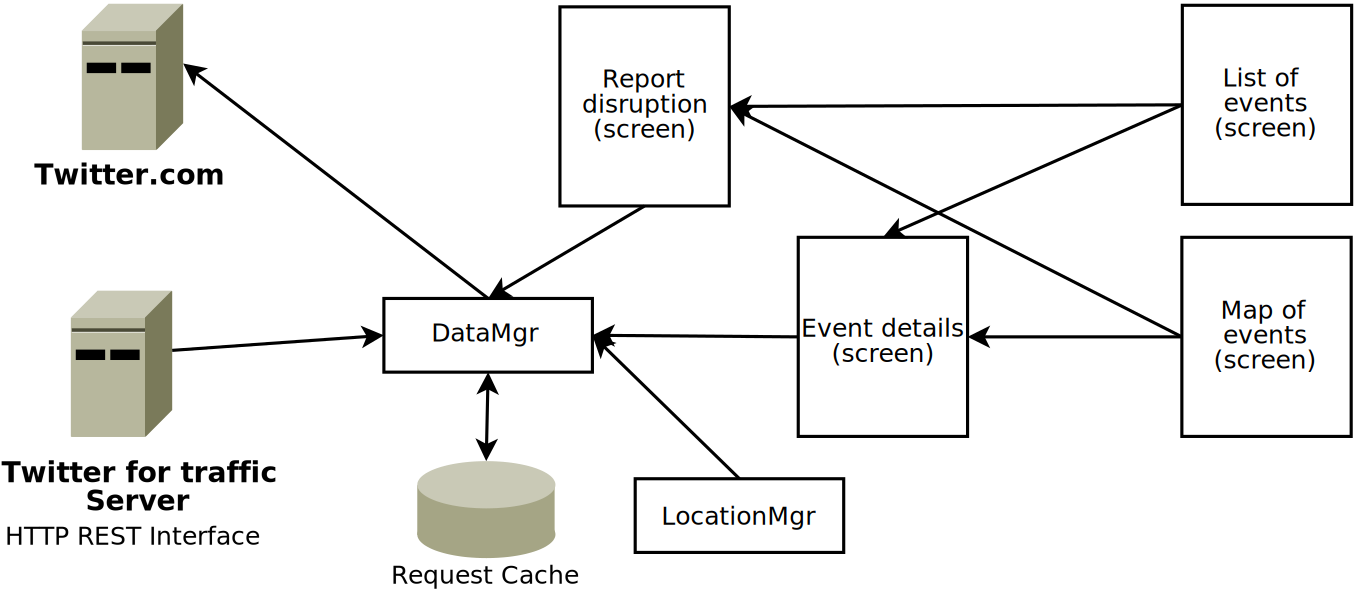
\includegraphics[width=0.9\textwidth]{images/design/client/client_high_level_layout.pdf}
\caption{High level client design}
\label{fig:client_design}
\end{figure}


\subsubsection{Server interface}
As previously discussed in this document, a ‘mock’ server was created to
parallelise efforts and to verify the REST endpoints. This tool proved very
useful in the development of the client application, particularly with verbose
logging on the server side when debugging connection issues.

The interaction with the server is encapsulated in the \emph{DataMgr} class.
This class returns lists of the relevant object types to the requester. The
interface for this class can be seen in Listing \ref{datamgrinterface}.

\lstset{caption={DataMgr.class public interface},label=datamgrinterface}

\begin{lstlisting}
public DataMgr(Context context);
public List<EventItem> requestEvents();
public List<TweetItem> requestTweets(String eventID);
public List<EventItem> requestRouteEvents(Route route);
\end{lstlisting}

\subsubsection{Request caching}
Modern mobile data networks have increased data-rates to an incredible level
over the last number of years, it is not uncommon now to see providers offering
speeds of up to 7.2 Mbps. But these types of networks also tend to incur large
latencies, for an initial TCP request from mobile handset round trip times of
up to one second are not unheard of.

As a mechanism to make the application feel more responsive to the user, a
cache of the response from the previous request is stored.

This cached response is displayed if the handset encounters one of two main
classes of problems. Firstly, in order to make a request for events in the
vicinity, we must request the current geographical location of the phone. If
the phones location cache is old or empty this request can take some time to
complete. Secondly, if the handset is experiencing difficulties connecting to
the server due to poor cellular connectivity. Once fresh data becomes available
the screen is populated with them. 

\subsubsection{Twitter interface}
To utilise Twitter for the reporting functionality, the JTwitter library from
Winterwell was used. This provided a simple interface to Twitter for our
application, enabling the posting of tweets as the signed in user and attaching
a geographical location to the tweet.

Using the library itself was trouble free, but Twitter recently moved
authentication for applications to Oauth. The Oauth protocol enables users to
authorise applications to access their account without providing the
applications with the users' login credentials, additionally it also enables
access restrictions to be applied on a per application basis.

The Oauth process for connecting a Twitter account uses the Oauth-Signpost
library and the resulting authorisation keys are saved in the application's
configuration. 

\subsubsection{Home route functionality}
A feature the team uncovered during the white boarding, was giving the user the
ability to store their typical route home from work. With this knowledge the
application could present the reported events that are relevant to the user.

The users configure the feature from the configuration screen, where they must
enter a postal address for their `home' and `work' locations. When the feature
is enabled and configured correctly, the map and list interfaces of the
application only display events within 300 meters of the route.

The feature relies on two features provided by Google, reverse geocoding
(address to geographical location) and requesting a driving route between two
geographical points. We start by requesting the best geographical point for the
`home' and `work' addresses. Following a successful response, we request a
driving route between those points. With this data we are able to draw the
route on the map and make a request to the server with the points on the route
for the relevant traffic events. The feature is illustrated in Figure~\ref{fig:home_route}.

\subsubsection{User interface}
As the Android client is the only user facing aspect of the system, it is
important to have a pleasant and intuitive user interface. To achieve this the
UI must behave as expected for that platform and features should require little
or no explanation regarding their operation. Following accepted Android design
patterns is a good way to attain this goal, the Android Development site
provides a good description of these principles \cite{website:android_ui}.

The interface was created over a number of revisions, with each one refining
and questioning the previous concepts. Some of these early designs are illustrated in
Figure \ref{fig:design_concepts} and examples of the final  user interface are in Figure
\ref{fig:user_interface}.
